\begin{figure}
\centering
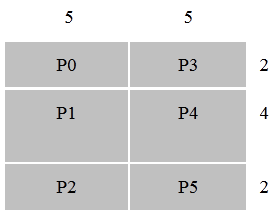
\includegraphics{CrIrreg}
\caption{Creating an Irregular Array}
\end{figure}


\begin{figure}
\centering
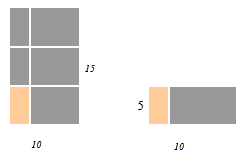
\includegraphics{GET}
\caption{Copying Data from 2-dimensional 15x10 Global Array into Local Buffer 5x10 Array}
\label{get}
\end{figure}

Figure \ref{get} shows the GET operation.

figure with label for referencing

Ordinary (inline) math mode. Mathematical material to be typeset inline must be surrounded by single dollar signs: "$a^2 + b^2 = c^2$". The dollar signs cause TeX to enter and exit (ordinary) math mode. 

display math mode

\[
a^2 + b^2 = c^2
\]


itemized list

\begin{itemize}
\item This is the first item
\item This is the second item
\item This is the last itme
\end{itemize}

If you have text that needs to look like code, you can use:

\begin{codeseg}
sample code
\end{codeseg}

\textless   -- gives you the less-than symbol
\codevar    -- gives you a chunk in "code-style" font ex:
\codevar{(ilo,jlo)}